% !TEX root = FDS_Validation_Guide.tex

\chapter{Suppression}

This chapter looks at validation exercises where the aim is to predict the extinguishment of a fire.

\section{Minimum Agent Concentration Experiments}

In the following sections, results of experiments are presented in which relatively small flames are extinguished due to the introduction of an inerting agent in the oxidizer stream.

\subsection{Cup Burner Experiments}
\label{Minimum Extinguishing Concentration}
A cup burner is an apparatus used to determine the minimum extinguishing concentration (MEC) for combinations of fuels and suppression agents. Sixteen fuels (acetone, acetylene, benzene, butane, dodecane, ethanol, ethylene, heptane, hexane, hydrogen, methane, methanol, octane, propane, propanol, and toluene) and five suppression agents (argon, carbon dioxide, helium, nitrogen, and sulfur hexaflouride) are considered. For the simulations, the MEC is found when the post-ignition HRR remains below $1 \times 10^{-10}$~kW. The critical flame temperatures specified for the fuel reactions are shown in Table~\ref{Cup_Table}. The extinguishing agent concentration is measured at the outer edge of the cup burner tube at a level slightly below the cup rim. Results are shown in Fig.~\ref{cup_burner_extinguish_vol} where color indicates the fuel and shape indicates the extinguishing agent.

\newpage

\begin{figure}[h!]
\begin{tabular*}{\textwidth}{l@{\extracolsep{\fill}}r}
\includegraphics[height=4in]{SCRIPT_FIGURES/ScatterPlots/FDS_Minimum_Extinguishing_Concentration} &
\raisebox{0.5\height}{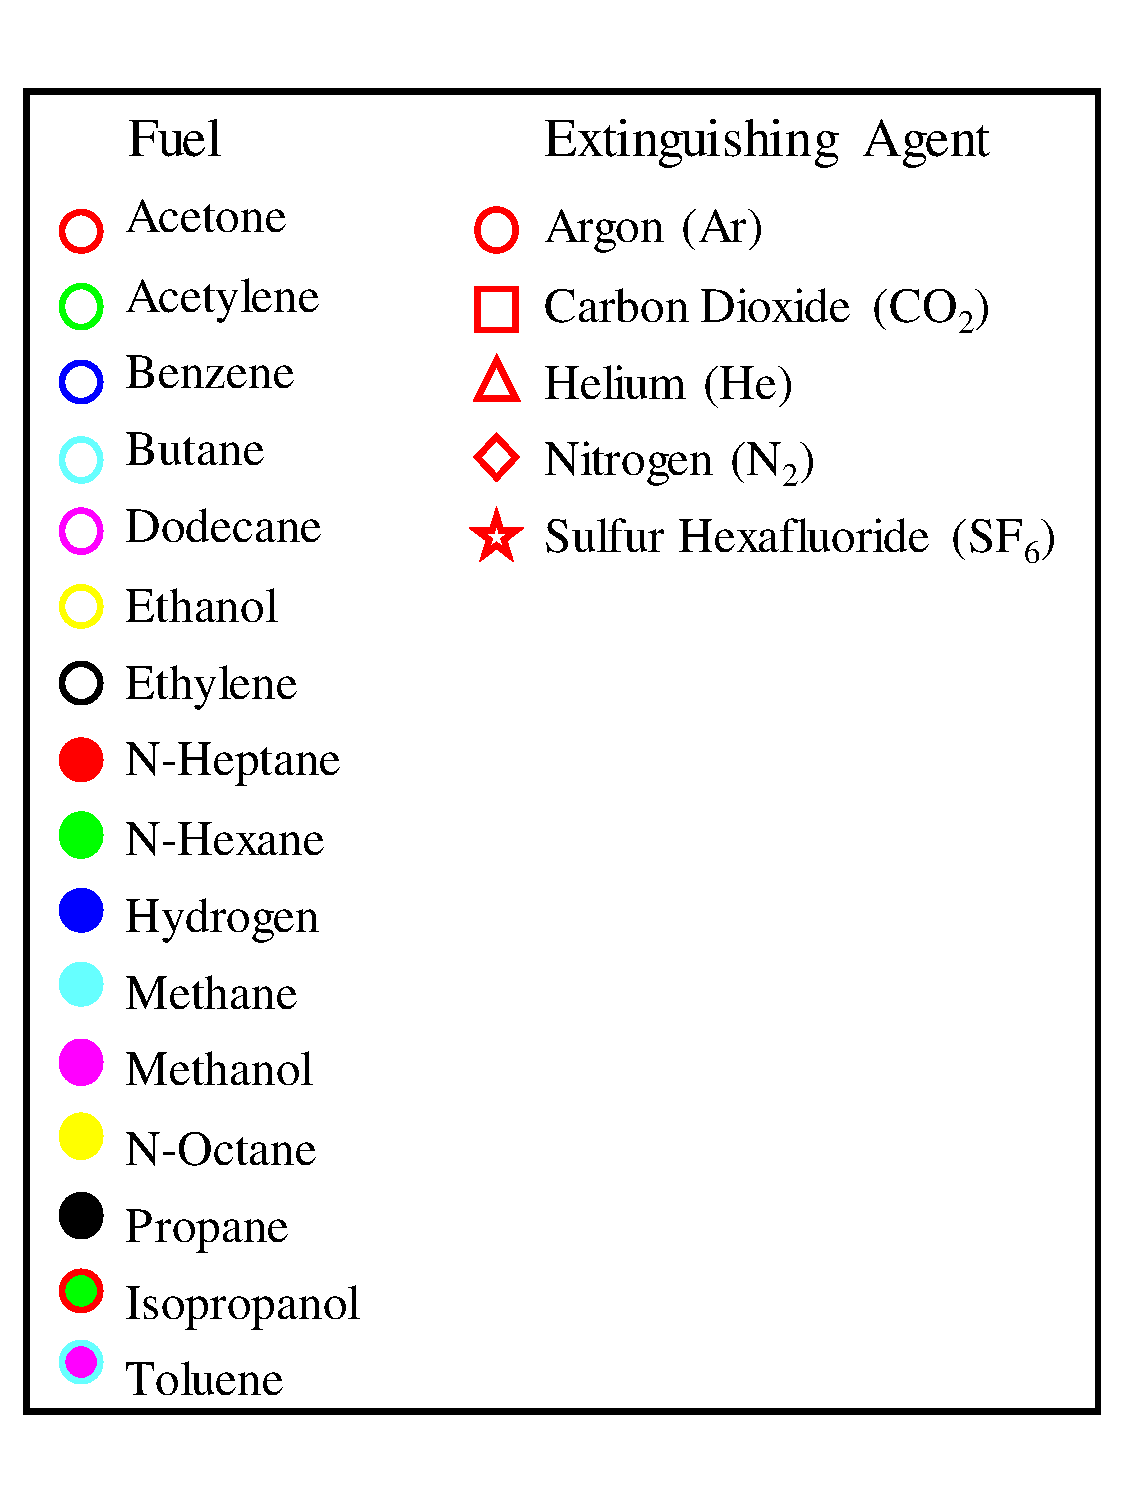
\includegraphics[height=2in]{FIGURES/Cup_Burner/Cup_Legend}}
\end{tabular*}
\caption[Results of Cup Burner experiments]{Comparison of measured and predicted minimum extinguishing volume fractions for the cup burner tests. Fuel type is indicated by color, and extinguishing agent is indicated by shape.}
\label{cup_burner_extinguish_vol}
\end{figure}

\clearpage

\subsection{FM Burner Experiments}

A description of the FM Burner experiments can be found in Section~\ref{FM_Burner_Description}. Briefly, a 15.2~cm round steel burner generating a 10~kW fire was supplied with oxygen by an air stream from below that was slowly diluted with nitrogen until the flame extinguished.  In the FDS simulations, nitrogen is added to the air stream supplied through the floor of the enclosure, linearly decreasing the oxygen volume fraction over one minute of simulated time. In Fig.~\ref{fig_fm_burner}, the combustion efficiency, $\eta$, is plotted as a function of oxygen volume fraction for all four fuels tested and compared with the measurements of Zeng and Wang~\cite{Zeng:26ICDERS}.  The auto-ignition temperature (AIT) threshold for each fuel is set according to the Beyler's chapter in the SFPE Handbook~\cite{SFPE:Beyler}.  The modeled burner is piloted using a ring of 36 hot (2000 \si{\degreeCelsius}) particles ejecting enough fuel to produce 1~kW (to match the experimental pilot).

\begin{figure}[!h]
\begin{tabular*}{\textwidth}{l@{\extracolsep{\fill}}r}
\includegraphics[height=2.1in]{SCRIPT_FIGURES/FM_Burner/eta_C2H4} &
\includegraphics[height=2.1in]{SCRIPT_FIGURES/FM_Burner/eta_C3H6} \\
\includegraphics[height=2.1in]{SCRIPT_FIGURES/FM_Burner/eta_C3H8} &
\includegraphics[height=2.1in]{SCRIPT_FIGURES/FM_Burner/eta_CH4}
\end{tabular*}
\caption[FM Burner combustion efficiency]{FM Burner combustion efficiency.}
\label{fig_fm_burner}
\end{figure}

\clearpage

\subsection{UMD Line Burner}

A description of UMD Line Burner experiments can be found in Section~\ref{UMD_Line_Burner_Description}. In the experiments, the oxygen co-flow was slowly diluted with nitrogen until the flame weakened and eventually extinguished.  In the FDS simulations, the nitrogen co-flow is setup with a ramp in time to achieve a linear decrease in the co-flow oxygen volume fraction over one minute of real time. In Fig.~\ref{fig_umd_comb_eta}, we plot the combustion efficiency as a function of oxygen volume fraction for both methane and propane and compare with the measurements of White~et~al.~\cite{White:2015}.  Note that the FDS results are presented for three different grid resolutions corresponding to $W/\delta x$ = 4, 8, and 16 ($\delta x$ = 1.25~cm, 0.625~cm, and 0.3125~cm, respectively), where $W=5$ cm is the width of the burner.  A simple re-ignition model with an ignition temperature threshold set to the SFPE Handbook~\cite{SFPE} value of the Auto-Ignition Temperature (AIT) for methane and propane is used.  A piloted ignition region (AIT = 0~K) is set just within the near field of the line burner.  Details of the re-ignition model and pilot region as well as parameter sensitivity studies are provided in White~et~al.~\cite{White:2017}.

\begin{figure}[!h]
\begin{tabular*}{\textwidth}{l@{\extracolsep{\fill}}r}
\includegraphics[height=2.1in]{SCRIPT_FIGURES/UMD_Line_Burner/methane_eta} &
\includegraphics[height=2.1in]{SCRIPT_FIGURES/UMD_Line_Burner/propane_eta}
\end{tabular*}
\caption[UMD Line Burner combustion efficiency]{UMD Line Burner combustion efficiency.}
\label{fig_umd_comb_eta}
\end{figure}

\clearpage


\section{Compartment Fire Extinction}

The following sections present results for experiments in which fires within forced ventilation compartments either self-extinguish due to lack of oxygen, or extinguish due to a water mist system.


\subsection{LLNL Enclosure Experiments}
\label{LLNL_Extinction Time}

The figures on the following pages contain plots of the heat release rate in both the experiments and the simulation. The experimental curve is just the value reported in the test report, which drops to zero instantly at the reported extinguishment time. In cases where the model does not predict extinction, the extinction time data is not used in the summary scatter plot, Fig.~\ref{USCG_Scatter}.

\newpage

\begin{figure}[p]
\begin{tabular*}{\textwidth}{l@{\extracolsep{\fill}}r}
\includegraphics[height=2.1in]{SCRIPT_FIGURES/LLNL_Enclosure/LLNL_Extinction_Test_1} &
\includegraphics[height=2.1in]{SCRIPT_FIGURES/LLNL_Enclosure/LLNL_Extinction_Test_2} \\
\includegraphics[height=2.1in]{SCRIPT_FIGURES/LLNL_Enclosure/LLNL_Extinction_Test_3} &
\includegraphics[height=2.1in]{SCRIPT_FIGURES/LLNL_Enclosure/LLNL_Extinction_Test_4} \\
\includegraphics[height=2.1in]{SCRIPT_FIGURES/LLNL_Enclosure/LLNL_Extinction_Test_5} &
\includegraphics[height=2.1in]{SCRIPT_FIGURES/LLNL_Enclosure/LLNL_Extinction_Test_6} \\
\includegraphics[height=2.1in]{SCRIPT_FIGURES/LLNL_Enclosure/LLNL_Extinction_Test_7} &
\includegraphics[height=2.1in]{SCRIPT_FIGURES/LLNL_Enclosure/LLNL_Extinction_Test_8}
\end{tabular*}
\caption[LLNL Extinction Time, Tests 1-8]{LLNL Extinction Time, Tests 1-8.}
\label{LLNL_Extinction_1}
\end{figure}

\begin{figure}[p]
\begin{tabular*}{\textwidth}{l@{\extracolsep{\fill}}r}
\includegraphics[height=2.1in]{SCRIPT_FIGURES/LLNL_Enclosure/LLNL_Extinction_Test_22} &
\includegraphics[height=2.1in]{SCRIPT_FIGURES/LLNL_Enclosure/LLNL_Extinction_Test_24} \\
\includegraphics[height=2.1in]{SCRIPT_FIGURES/LLNL_Enclosure/LLNL_Extinction_Test_25} &
\includegraphics[height=2.1in]{SCRIPT_FIGURES/LLNL_Enclosure/LLNL_Extinction_Test_27} \\
\includegraphics[height=2.1in]{SCRIPT_FIGURES/LLNL_Enclosure/LLNL_Extinction_Test_28} &
\includegraphics[height=2.1in]{SCRIPT_FIGURES/LLNL_Enclosure/LLNL_Extinction_Test_29} \\
\includegraphics[height=2.1in]{SCRIPT_FIGURES/LLNL_Enclosure/LLNL_Extinction_Test_32} &
\includegraphics[height=2.1in]{SCRIPT_FIGURES/LLNL_Enclosure/LLNL_Extinction_Test_37}
\end{tabular*}
\caption[LLNL Extinction Time, Tests 22, 24, 25, 27, 28, 29, 32, 37]
{LLNL Extinction Time, Tests 22, 24, 25, 27, 28, 29, 32, 37.}
\label{LLNL_Extinction_2}
\end{figure}

\begin{figure}[p]
\begin{tabular*}{\textwidth}{l@{\extracolsep{\fill}}r}
\includegraphics[height=2.1in]{SCRIPT_FIGURES/LLNL_Enclosure/LLNL_Extinction_Test_39} &
\includegraphics[height=2.1in]{SCRIPT_FIGURES/LLNL_Enclosure/LLNL_Extinction_Test_41} \\
\includegraphics[height=2.1in]{SCRIPT_FIGURES/LLNL_Enclosure/LLNL_Extinction_Test_43} &
\includegraphics[height=2.1in]{SCRIPT_FIGURES/LLNL_Enclosure/LLNL_Extinction_Test_44} \\
\includegraphics[height=2.1in]{SCRIPT_FIGURES/LLNL_Enclosure/LLNL_Extinction_Test_45} &
\includegraphics[height=2.1in]{SCRIPT_FIGURES/LLNL_Enclosure/LLNL_Extinction_Test_46} \\
\includegraphics[height=2.1in]{SCRIPT_FIGURES/LLNL_Enclosure/LLNL_Extinction_Test_47} &
\includegraphics[height=2.1in]{SCRIPT_FIGURES/LLNL_Enclosure/LLNL_Extinction_Test_48}
\end{tabular*}
\caption[LLNL Extinction Time, Tests 39, 41, 43-48]
{LLNL Extinction Time, Tests 39, 41, 43-48.}
\label{LLNL_Extinction_3}
\end{figure}

\begin{figure}[p]
\begin{tabular*}{\textwidth}{l@{\extracolsep{\fill}}r}
\includegraphics[height=2.1in]{SCRIPT_FIGURES/LLNL_Enclosure/LLNL_Extinction_Test_49} &
\end{tabular*}
\caption[LLNL Extinction Time, Test 49]{LLNL Extinction Time, Test 49.}
\label{LLNL_Extinction_4}
\end{figure}

\clearpage


\subsection{SWJTU Tunnel Experiments}

The figures below display the heat release rate as a function of time for the SWJTU Tunnel experiments.

\begin{figure}[!h]
\begin{tabular*}{\textwidth}{l@{\extracolsep{\fill}}r}
\includegraphics[height=2.1in]{SCRIPT_FIGURES/SWJTU_Tunnels/Test_I-1_Ext_Time} &
\includegraphics[height=2.1in]{SCRIPT_FIGURES/SWJTU_Tunnels/Test_I-2_Ext_Time} \\
\includegraphics[height=2.1in]{SCRIPT_FIGURES/SWJTU_Tunnels/Test_I-3_Ext_Time} &
\includegraphics[height=2.1in]{SCRIPT_FIGURES/SWJTU_Tunnels/Test_I-4_Ext_Time} \\
\includegraphics[height=2.1in]{SCRIPT_FIGURES/SWJTU_Tunnels/Test_I-5_Ext_Time} &
\includegraphics[height=2.1in]{SCRIPT_FIGURES/SWJTU_Tunnels/Test_I-6_Ext_Time}
\end{tabular*}
\caption[SWJTU Tunnel experiments, extinction time]{SWJTU Tunnel experiments, extinction time.}
\label{SWJTU_Extinction}
\end{figure}


\clearpage


\subsection{USCG/HAI Water Mist Suppression Tests}

The following pages contain comparisons of the predicted heat release rates for fires that are suppressed with a water mist system. In all cases, the flow rate of liquid fuel is specified in the model, but the decrease in HRR due to the extinguishing system is predicted by the model. Table~\ref{USCG_HAI_Times} reports the observed extinguishment times. Figure~\ref{USCG_Scatter} compares the measured versus predicted extinguishment times. For the simulations, the extinguishment time is taken to be when the HRR drops to half of its specified value.

In cases where there is no reported fire extinction or the model does not predict extinction, the extinction time data is not used in the summary scatter plot, Fig.~\ref{USCG_Scatter}.


\begin{table}[h!]
\caption[USCG/HAI water mist suppression extinguishment times]{Recorded extinguishment times for the USCG/HAI water mist suppression tests in a small shipboard machinery space. ``No''
means that the fire was not extinguished within 600 s of nozzle activation.}
\begin{center}
\begin{tabular}{|l|c|c|c|c|c|c|}
\hline
\multicolumn{2}{|l|}{System}                            & Navy  & Grinnell  & Fogtec    & Chemetron & Fike   \\ \hline  \hline
\multicolumn{2}{|l|}{Number of Nozzles}                 & 6     & 6         & 6         & 15        & 6      \\ \hline
\multicolumn{2}{|l|}{Operating Pressure (bar)}          & 70    & 13        & 100       & 12        & 21     \\ \hline
\multicolumn{2}{|l|}{Flow Rate (L/min)}                 & 68    & 75        & 22        & 70        & 48     \\ \hline
\multicolumn{2}{|l|}{Assumed Median Drop Size ($\mu$m)} & 175   & 225       & 100       &           & 200    \\ \hline
\multicolumn{2}{|l|}{Assumed Initial Velocity (m/s)}    & 75    & 32        & 90        &           & 41     \\ \hline
\multicolumn{2}{|l|}{Assumed Spray Angle (deg.)}        & 120   & 90        & 120       &           & 90     \\ \hline \hline
Fire Scenario       & Ventilation                       & \multicolumn{5}{c|}{Extinguishment Time (s)}      \\ \hline \hline
1.0 MW Spray        & Closed                            & 15    & 26        & 21        & 27        & 21     \\ \hline
1.0 MW Spray        & Natural                           & 15    & 40        & 32        & 43        & 35     \\ \hline
1.0 MW Spray        & Forced                            & 17    & 55        & 76        & 357       & 133    \\ \hline
0.5 MW Spray        & Closed                            & 34    & 70        & 39        & 53        & 56     \\ \hline
0.5 MW Spray        & Natural                           & 41    & 117       & 67        & 158       & 140    \\ \hline
0.5 MW Spray        & Forced                            & 124   & No        & No        & No        & No     \\ \hline
0.25 MW Spray       & Closed                            & 157   & 360       & 169       & 314       & 277    \\ \hline
0.25 MW Spray       & Natural                           & 206   & No        & 290       & 525       & 566    \\ \hline
0.25 MW Spray       & Forced                            & No    & No        & No        & No        & No     \\ \hline
\end{tabular}
\end{center}
\label{USCG_HAI_Times}
\end{table}



\newpage

\begin{figure}[p]
\begin{tabular*}{\textwidth}{l@{\extracolsep{\fill}}r}
\includegraphics[height=2.1in]{SCRIPT_FIGURES/USCG_HAI/USCG_HAI_HRR_1000_Closed_Grinnell} &
\includegraphics[height=2.1in]{SCRIPT_FIGURES/USCG_HAI/USCG_HAI_HRR_1000_Closed_Navy} \\
\includegraphics[height=2.1in]{SCRIPT_FIGURES/USCG_HAI/USCG_HAI_HRR_1000_Closed_Fogtec} &
\includegraphics[height=2.1in]{SCRIPT_FIGURES/USCG_HAI/USCG_HAI_HRR_1000_Closed_Fike} \\
\includegraphics[height=2.1in]{SCRIPT_FIGURES/USCG_HAI/USCG_HAI_HRR_1000_Natural_Grinnell} &
\includegraphics[height=2.1in]{SCRIPT_FIGURES/USCG_HAI/USCG_HAI_HRR_1000_Natural_Navy} \\
\includegraphics[height=2.1in]{SCRIPT_FIGURES/USCG_HAI/USCG_HAI_HRR_1000_Natural_Fogtec} &
\includegraphics[height=2.1in]{SCRIPT_FIGURES/USCG_HAI/USCG_HAI_HRR_1000_Natural_Fike}
\end{tabular*}
\caption[USCG/HAI experiments, extinction time]{USCG/HAI experiments, extinction time.}
\label{USCG_HAI_2}
\end{figure}

\begin{figure}[p]
\begin{tabular*}{\textwidth}{l@{\extracolsep{\fill}}r}
\includegraphics[height=2.1in]{SCRIPT_FIGURES/USCG_HAI/USCG_HAI_HRR_1000_Forced_Grinnell} &
\includegraphics[height=2.1in]{SCRIPT_FIGURES/USCG_HAI/USCG_HAI_HRR_1000_Forced_Navy} \\
\includegraphics[height=2.1in]{SCRIPT_FIGURES/USCG_HAI/USCG_HAI_HRR_1000_Forced_Fogtec} &
\includegraphics[height=2.1in]{SCRIPT_FIGURES/USCG_HAI/USCG_HAI_HRR_1000_Forced_Fike} \\
\includegraphics[height=2.1in]{SCRIPT_FIGURES/USCG_HAI/USCG_HAI_HRR_500_Closed_Grinnell} &
\includegraphics[height=2.1in]{SCRIPT_FIGURES/USCG_HAI/USCG_HAI_HRR_500_Closed_Navy} \\
\includegraphics[height=2.1in]{SCRIPT_FIGURES/USCG_HAI/USCG_HAI_HRR_500_Closed_Fogtec} &
\includegraphics[height=2.1in]{SCRIPT_FIGURES/USCG_HAI/USCG_HAI_HRR_500_Closed_Fike}
\end{tabular*}
\caption[USCG/HAI experiments, extinction time]{USCG/HAI experiments, extinction time.}
\label{USCG_HAI_4}
\end{figure}

\begin{figure}[p]
\begin{tabular*}{\textwidth}{l@{\extracolsep{\fill}}r}
\includegraphics[height=2.1in]{SCRIPT_FIGURES/USCG_HAI/USCG_HAI_HRR_500_Natural_Grinnell} &
\includegraphics[height=2.1in]{SCRIPT_FIGURES/USCG_HAI/USCG_HAI_HRR_500_Natural_Navy} \\
\includegraphics[height=2.1in]{SCRIPT_FIGURES/USCG_HAI/USCG_HAI_HRR_500_Natural_Fogtec} &
\includegraphics[height=2.1in]{SCRIPT_FIGURES/USCG_HAI/USCG_HAI_HRR_500_Natural_Fike} \\
\includegraphics[height=2.1in]{SCRIPT_FIGURES/USCG_HAI/USCG_HAI_HRR_500_Forced_Grinnell} &
\includegraphics[height=2.1in]{SCRIPT_FIGURES/USCG_HAI/USCG_HAI_HRR_500_Forced_Navy} \\
\includegraphics[height=2.1in]{SCRIPT_FIGURES/USCG_HAI/USCG_HAI_HRR_500_Forced_Fogtec} &
\includegraphics[height=2.1in]{SCRIPT_FIGURES/USCG_HAI/USCG_HAI_HRR_500_Forced_Fike}
\end{tabular*}
\caption[USCG/HAI experiments, extinction time]{USCG/HAI experiments, extinction time.}
\label{USCG_HAI_6}
\end{figure}

\begin{figure}[p]
\begin{tabular*}{\textwidth}{l@{\extracolsep{\fill}}r}
\includegraphics[height=2.1in]{SCRIPT_FIGURES/USCG_HAI/USCG_HAI_HRR_250_Closed_Grinnell} &
\includegraphics[height=2.1in]{SCRIPT_FIGURES/USCG_HAI/USCG_HAI_HRR_250_Closed_Navy} \\
\includegraphics[height=2.1in]{SCRIPT_FIGURES/USCG_HAI/USCG_HAI_HRR_250_Closed_Fogtec} &
\includegraphics[height=2.1in]{SCRIPT_FIGURES/USCG_HAI/USCG_HAI_HRR_250_Closed_Fike} \\
\includegraphics[height=2.1in]{SCRIPT_FIGURES/USCG_HAI/USCG_HAI_HRR_250_Natural_Grinnell} &
\includegraphics[height=2.1in]{SCRIPT_FIGURES/USCG_HAI/USCG_HAI_HRR_250_Natural_Navy} \\
\includegraphics[height=2.1in]{SCRIPT_FIGURES/USCG_HAI/USCG_HAI_HRR_250_Natural_Fogtec} &
\includegraphics[height=2.1in]{SCRIPT_FIGURES/USCG_HAI/USCG_HAI_HRR_250_Natural_Fike}
\end{tabular*}
\caption[USCG/HAI experiments, extinction time]{USCG/HAI experiments, extinction time.}
\label{USCG_HAI_8}
\end{figure}


\begin{figure}[p]
\begin{tabular*}{\textwidth}{l@{\extracolsep{\fill}}r}
\includegraphics[height=2.1in]{SCRIPT_FIGURES/USCG_HAI/USCG_HAI_HRR_250_Forced_Grinnell} &
\includegraphics[height=2.1in]{SCRIPT_FIGURES/USCG_HAI/USCG_HAI_HRR_250_Forced_Navy} \\
\includegraphics[height=2.1in]{SCRIPT_FIGURES/USCG_HAI/USCG_HAI_HRR_250_Forced_Fogtec} &
\includegraphics[height=2.1in]{SCRIPT_FIGURES/USCG_HAI/USCG_HAI_HRR_250_Forced_Fike}
\end{tabular*}
\caption[USCG/HAI experiments, extinction time]{USCG/HAI experiments, extinction time.}
\label{USCG_HAI_9}
\end{figure}

\clearpage

\subsection{Summary, Flame Extinction Time}
\label{Extinction Time}

\begin{figure}[h!]
\begin{center}
\includegraphics[height=4in]{SCRIPT_FIGURES/ScatterPlots/FDS_Extinction_Time}
\caption[Extinguishment times for the USCG/HAI water mist suppression tests]{Comparison of measured and predicted extinguishment times for the USCG/HAI water mist suppression tests.}
\label{USCG_Scatter}
\end{center}
\end{figure}

\clearpage

\section{VTT Water Spray Experiments}

Figure~\ref{LN02} presents profiles of mean droplet diameter, mean velocity, and droplet flux below a single 74$^\circ$ hollow-cone water mist nozzle. The pressure behind the nozzle was 2~MPa, and the flow constant was 0.077~L/min/bar$^{1/2}$. The The experimental data represents average values at each distance calculated over the four measuring points at that distance (except for the point at the spray axis). A comparison of droplet speed, mist flux and Sauter mean diameter ($D_{32}$) profiles are shown in Fig.~\ref{LN02}. Comparisons are shown at 40~cm and 62~cm vertical distances from the nozzle. Simulation results are reported for three spatial resolutions: 1~cm, 2~cm, and 4~cm.

\begin{figure}
\begin{tabular*}{\textwidth}{l@{\extracolsep{\fill}}r}
\includegraphics[height=2.1in]{SCRIPT_FIGURES/VTT_Sprays/LN02_velo_40} &
\includegraphics[height=2.1in]{SCRIPT_FIGURES/VTT_Sprays/LN02_velo_62}  \\
\includegraphics[height=2.1in]{SCRIPT_FIGURES/VTT_Sprays/LN02_flux_40} &
\includegraphics[height=2.1in]{SCRIPT_FIGURES/VTT_Sprays/LN02_flux_62}  \\
\includegraphics[height=2.1in]{SCRIPT_FIGURES/VTT_Sprays/LN02_diam_40} &
\includegraphics[height=2.1in]{SCRIPT_FIGURES/VTT_Sprays/LN02_diam_62}  \\
\end{tabular*}
\caption[Droplet speed, flux, and mean diameter profiles of the LN-2 nozzle]{Comparison of predicted and experimental droplet speed (top), droplet flux (middle) and mean diameter (bottom) profiles of the LN-2 nozzle. The left column corresponds to measurements made 40~cm from the nozzle, while the right column corresponds to measurements made 62~cm from the nozzle.}
\label{LN02}
\end{figure}

